\chapter{Challenges for Design of Applications}
The biggest design challenge for developers of gesture controls is market adoption, standardization and gesture choice. From getting users to use the technology to make the technology comfortable to use on a daily basis. Developers both in hardware and software face many challenges in developing with this technology.

\section{Market Adoption}

\subsection{Myo Armband}

\begin{wrapfigure}{r}{0.5\textwidth}
  \begin{center}
    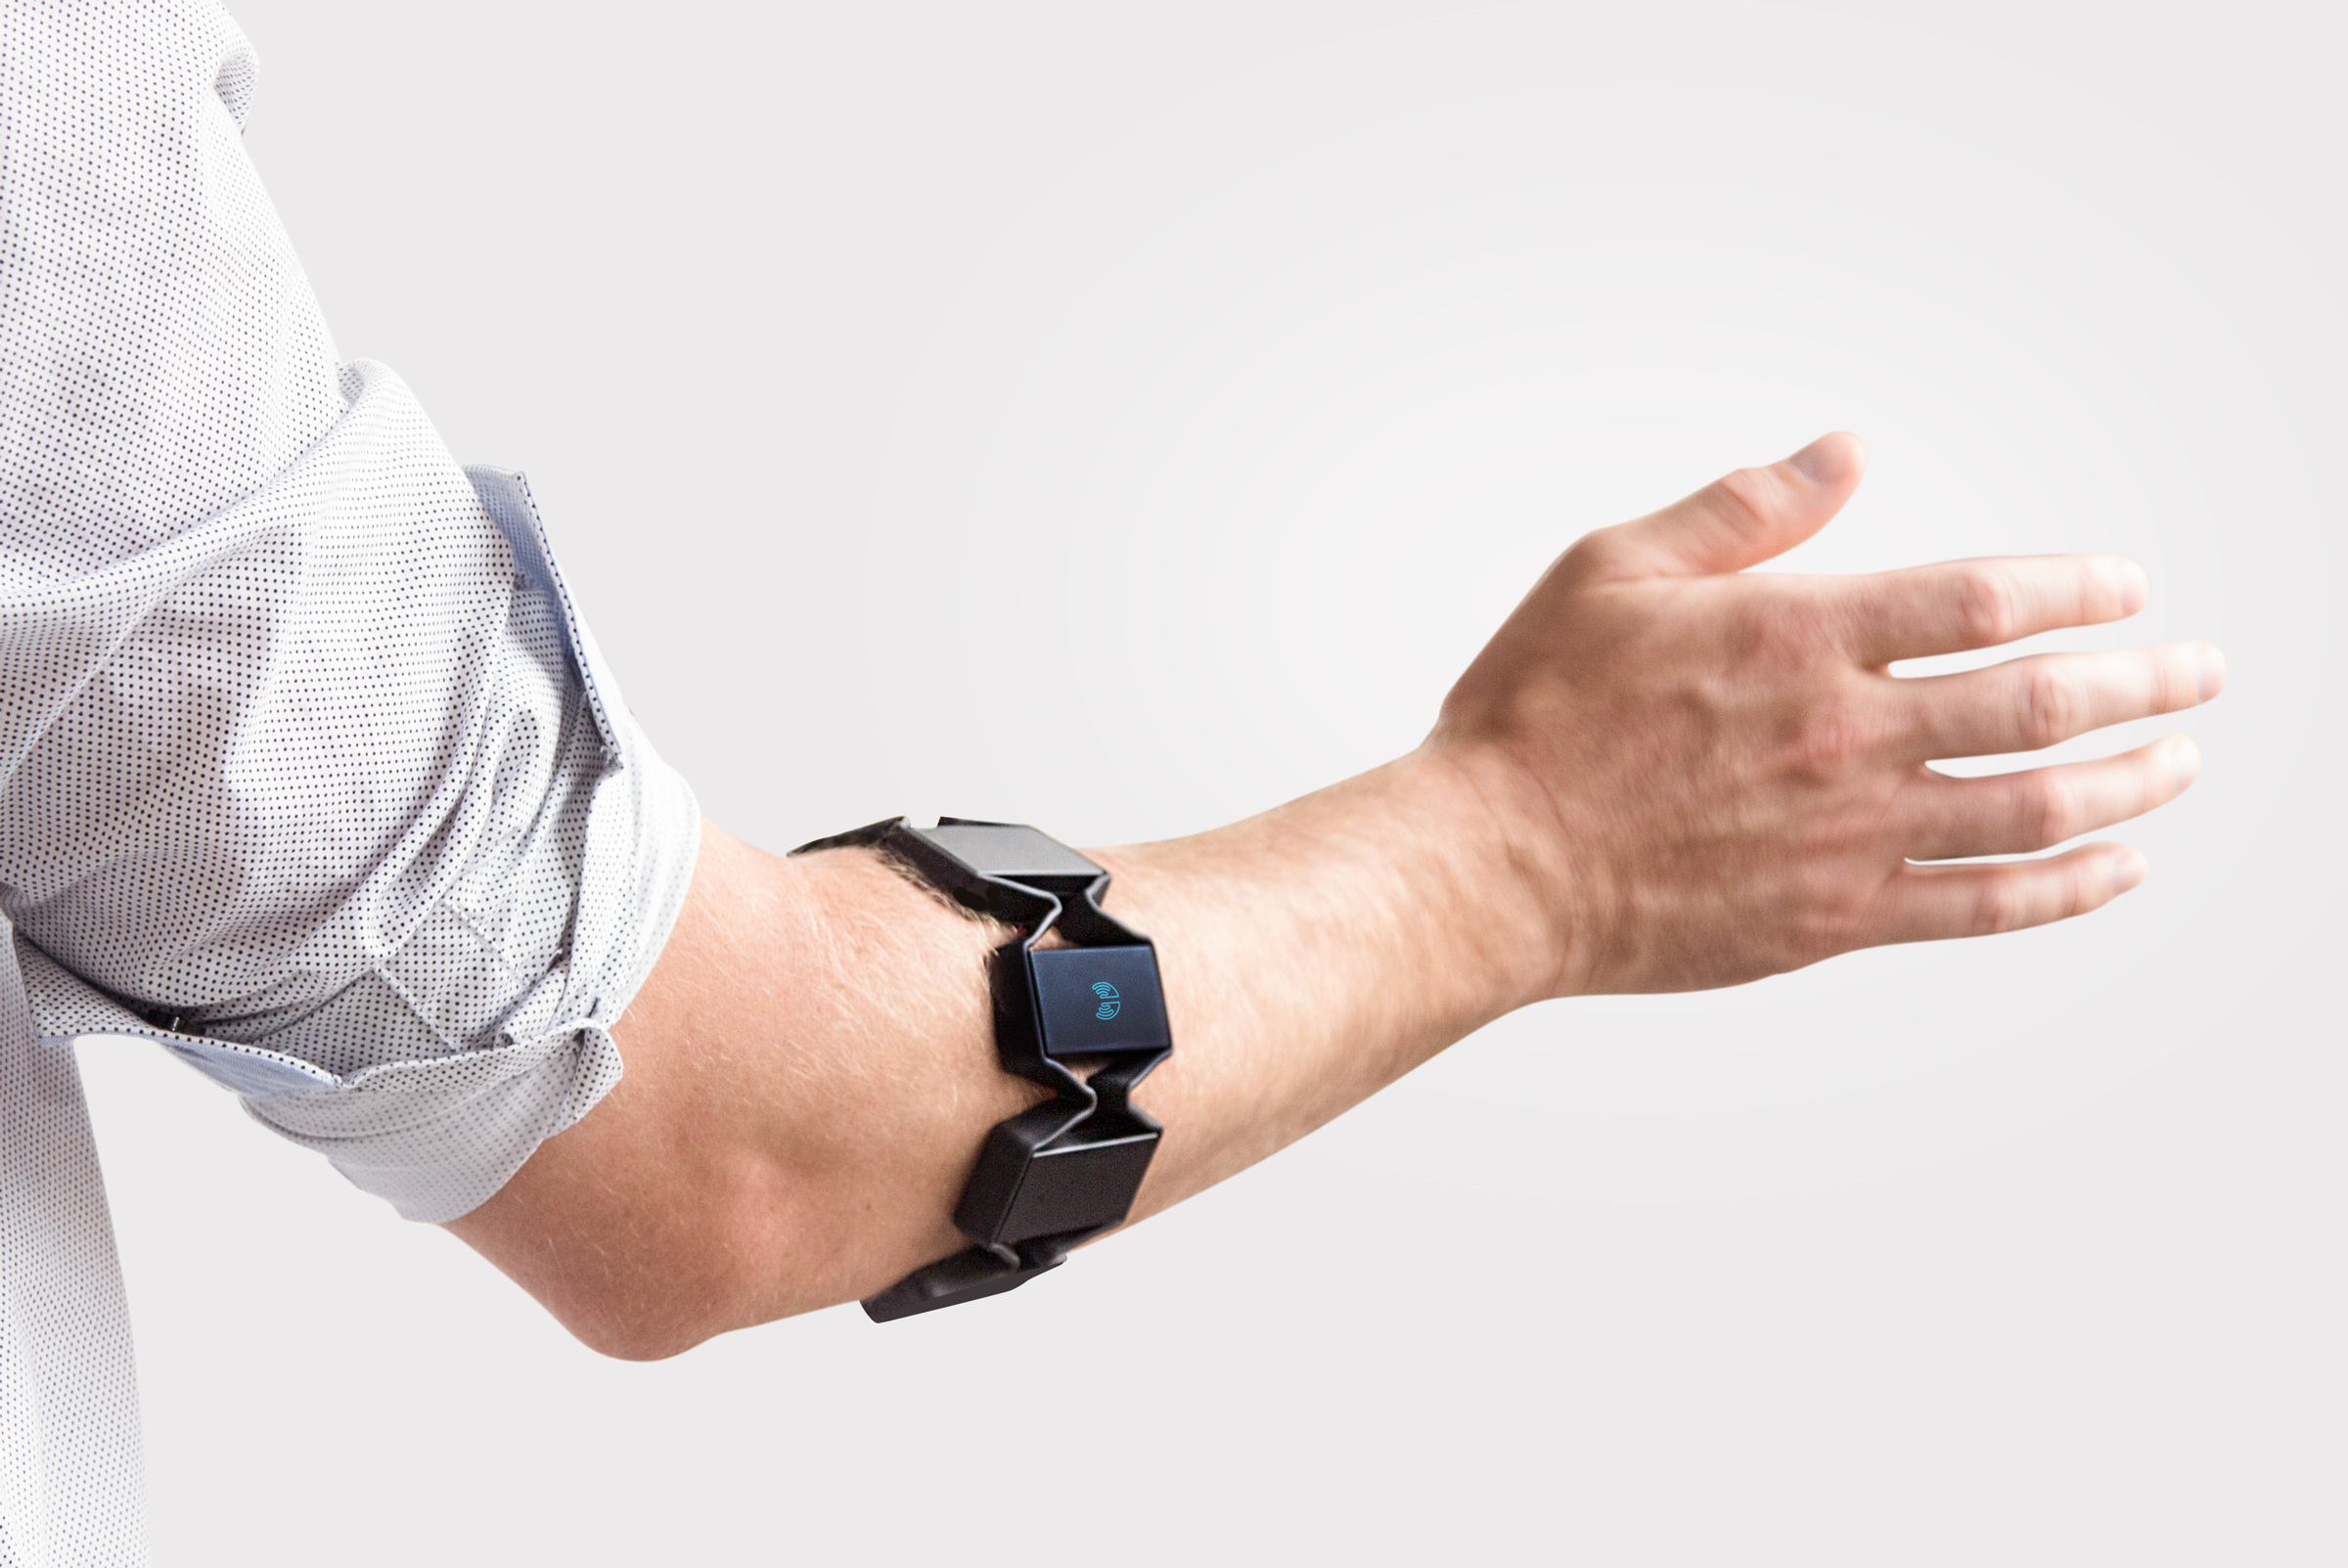
\includegraphics[width=0.48\textwidth]{img/myo.jpg}
  \end{center}
  \caption{Myo Armband}
\end{wrapfigure}

One of the biggest challenges of gesture-based technology is market adoption. If the technology isn't adopted by a large segment of the population developers mostly ignore it in favour of a bigger market, such as mobile phones and the traditional desktop.

Devices like the Myo armband started out with great success raising 14.5 Million dollars in 2013 with 30,000 pre-orders for their product. The problem started with lacklustre support from developers who weren't as supportive of the technology as the customers were. \cite{myosales}

Devices like Myo Armband suffered due to developer support which caused customers to lose interest with the technology.

\subsection{Kinect}
Even industry giant Microsoft tried to break into the gesture controls space with the introduction of the Kinect back in 2010. \cite{kinect} The Kinect was Microsoft's attempt of adding gesture controls to their gaming console the Xbox 360. With support from Microsoft, many developers made Kinect only games (Kinect Sports, Kinect Adventures!, Kinectimals) and other added Kinect support (Elder Scrolls: Skyrim, Forza Motorsports 4). With support from Microsoft, the Kinect looked to be on the rise as sales reached 10 Million. \cite{kinectsales}

\begin{figure}[H]
  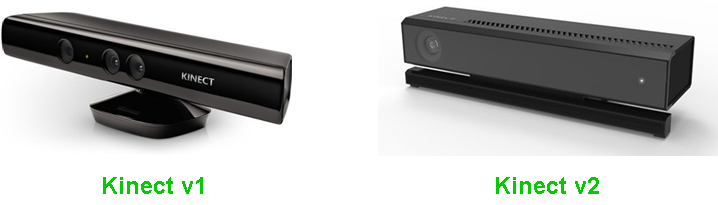
\includegraphics[width=\linewidth]{img/Kinect.png}
  \caption{Kinect V1/2}
  \label{fig:KINECT}
\end{figure}

From 2010 (Release of Kinect V1) to 2013 (Release of Kinect V2) customers opinion had changed on the Kinect. Many felt the Kinect games felt gimmicky' and games that added Kinect support didn't make using it over a traditional controller better. This dislike of gesture controls came to ahead with the release of the Xbox One, which originally was debuted with a new Kinect, which had to be plugged in at all times. With a price tag 100 dollars more than their competition, many blamed the Kinect for this price difference. 

With the Xbox One release having a Kinect market adaption should have been even better than the previous iteration of the Kinect. Unfortunately, the announcement of the Xbox One was a disaster causing lots of controversies that was then directed towards the Kinect. The Kinect got lacklustre support and many had a concern of privacy with an always-on camera and speaker. The Kinect was dropped in later models of Xbox Ones with users having to buy an adapter to get one to work with the newer models. This adapter was then dropped leaving users who enjoyed the connect behind.

\section{Standardization}
A huge problem with gesture controls is standardizing the technology involved. Each company makes its own proprietary technology which leads to lacklustre developer support if the consumer-base isn't high enough. An example is the Xbox Kinect. The Kinect got support from Microsoft with games only for Kinect, which is fine as the game is developed by Microsoft. The problem with support comes from third party companies. These companies want the biggest profit they can get and by creating a Kinect only game it restricts their consumer-base to Kinect only users. Companies would rather release on both Xbox and PlayStation and add in Kinect features. The problem with this style of development is it leads to these Kinect features being thought of after the game has already been made, leading them to be pushed to the side as 'gimmicky' by consumers.

Microsoft is trying to create a standard using their Microsoft Launcher on Android Phones. By allowing the user to customize what gestures do for them, making the gestures more comfortable for the user and by putting this feature on the Android Play-Store giving users around the world access to this feature set.

\section{Gesture Choice}
During the development of gesture-based technology, the developers need to be wary of how the gestures are used. Gestures that mean one thing here means something else over there, so if developers aren't careful they can be met with lots of criticism. A huge part of gesture development is researching the gesture controls to see which gesture would fit best for a particular action.

With less and fewer buttons on phones, many developers have to keep gestures in mind when developing applications for phones. Luckily both Android and iPhone share similar designs allowing developers to carry these gestures across devices, hitting a larger market of users. Phones are a word wide item used by billions. Many people take gestures on phones for granted as we become accustomed to them. If an application doesn't support basic gestures such as swiping up and down to navigate it can make it feel quite old and awkward to use so many will just not use it.

An important part of developing gestures for users is to keep some sort of standard. Many expect to be able to swipe up and down to navigate with one finger, changing this to require two for your application will annoy user away from it. This is why hardware manufacturers like Apple will include how developers should handle certain gestures. 